\chapter{Experiment and Application Design}




This chapter describes the design of the experiment framework, both the experiment and the application side.
The application will be explained from the system design point-of-view and the user experience perspective. First,
The application high-level decision and work flow are explained using a flow chart and a class diagram.



\section{Experiment design}
\subsection{Participant}
21 Participants are participated in the study. All of the participant are student of University of Edinburgh.
3 students participate as a tester to ensure the application works perfectly. While 18 students conducted the experiment, and their data are analyzed.

\subsection{Procedure}
The experiment is conducted as a form of quiz where a number of questions is presented to the participant and the participant need to look the answer in the answer page.
More detailed about the experiment can bee seen on experiment design section.

Three studies are conducted. On each study, 10 questions with the same category will be presented to the participant. The study is conducted in a silent lab
 room in a forrest hill lab and a meeting room on the library. The room is kept empty and quite to lower the level distraction.

These studies are explained below;
\begin{itemize}
\item study 1 : one question at a time will be presented to 4 participants.
\item study 2 : one or two questions at a time will be presented to 11 participants.
\item study 3 : one question is presented to 3 participants. every time a participant look at the question he/she is instructed to move to another the room.
\end{itemize}

\subsection{Question}
During the experiment 10 questions are used. The questions are designed as simple as possible so it does not require the participant to remember long context of the question.
The questions and its answer are listed on the table \ref{tab:questions}

% \begin{table}[!h]
%   \centering
% \begin{longtable}{|p{0.5cm}|p{4.5cm}|p{7cm}|p{3cm}|  }
%  \hline
%  No& Question & Answer link & Asnwer \\
%  \hline
%  1 & What is the original name of the titanic movie ?  & https://www.simplemost.com/15-fun-facts-probably-didnt-know-titanic/ & Planet ice\\
%  2 & In the movie "Lord of the Rings", How tall is Gandalf ? & https://www.phactual.com/14-fun-facts-about-the-lord-of-the-rings-the-fellowship-of-the-ring/ & Seven foot\\
%  3 & How many actors played both in Game of Thrones and in the Harry Potter movies ? & http://screenrant.com/best-facts-game-of-thrones-trivia/ & 9\\
%  4 & What is the meaning of Dumbledore in the Harry Potter movies ? & http://www.teenvogue.com/gallery/harry-potter-facts & Bumbelbee \\
%  5 & How many years has “How i met your mother” been filmed ? & https://www.phactual.com/10-fun-facts-about-how-i-met-your-mother/ & 9 years \\
%  6 &  How many baloons are attached to carl’s house in the "UP" movie ? & https://filmschoolrejects.com/10-fun-facts-about-pixars-up-1749a61575ca/ & 10,297 \\
%  7 & Where does marvel get the idea of the black spiderman suit ? & http://screenrant.com/best-marvel-facts-trivia-movies-tv-comics-superheroes/ & Fan or Randy \\
%  8 & What is the most expensive movie of all time ? & https://www.factretriever.com/hollywood-movies-facts & Avatar\\
%  9 & How many academy awards has the movie "UP" been nominated to ? &  http://www.imdb.com/title/tt1049413/trivia & two \\
% 10 & What is the most watched episode on the show “How i met your mother” ? & https://ritely.com/how-i-met-your-mother-trivia/ & The finale episode \\
%    \hline
% \end{longtable}
%  \caption{The questions used in the experiment}
%  \label{tab:questions}
% \end{table}

\begin{table}[!b]
\centering
\small
\footnotesize
\setlength\tabcolsep{2pt}
\begin{tabu}to \textwidth {|X[0.5,l]|
							X[5,l]|
                            X[7,l]|
                            X[2.8,l]|}
\hline
No & Question                                                                        & Answer Link                                                                                   & Answer             \\ \hline
1  & What is the original name of the titanic movie ?                                & https://www.simplemost.com/15-fun-facts-probably-didnt-know-titanic/                          & Planet             \\ \hline
2  & In the movie "Lord of the Rings", How tall is Gandalf ?                         & https://www.phactual.com/14-fun-facts-about-the-lord-of-the-rings-the-fellowship-of-the-ring/ & Seven foot         \\ \hline
3  & How many actors played both in Game of Thrones and in the Harry Potter movies ? & http://screenrant.com/best-facts-game-of-thrones-trivia/                                      & 9                  \\ \hline
4  & What is the meaning of Dumbledore in the Harry Potter movies ?                  & http://www.teenvogue.com/gallery/harry-potter-facts                                           & Bumbelbee          \\ \hline
5  & How many years has “How i met your mother” been filmed ?                        & https://www.phactual.com/10-fun-facts-about-how-i-met-your-mother/                            & 9 years            \\ \hline
6  & How many baloons are attached to carl’s house in the "UP" movie ?               & https://filmschoolrejects.com/10-fun-facts-about-pixars-up-1749a61575ca/                      & 10,297             \\ \hline
7  & Where does marvel get the idea of the black spiderman suit ?                    & http://screenrant.com/best-marvel-facts-trivia-movies-tv-comics-superheroes/                  & Fan or Randy       \\ \hline
8  & What is the most expensive movie of all time ?                                  & https://www.factretriever.com/hollywood-movies-facts                                          & Avatar             \\ \hline
9  & How many academy awards has the movie "UP" been nominated to ?                  & http://www.imdb.com/title/tt1049413/trivia                                                    & two                \\ \hline
10 & What is the most watched episode on the show “How i met your mother” ?          & https://ritely.com/how-i-met-your-mother-trivia/                                              & The finale episode \\ \hline
\end{tabu}
 \caption{The questions used in the experiment}
 \label{tab:questions}
\end{table}


\subsection{Demographic question}
The participant is required to answer demographic questions at the end of the experiment.
The list of the demographic questions can be seen on the table \ref{tab:demographicQuestion}

\begin{table}[!b]
  \centering
  \small
  \footnotesize
\begin{tabu}{ |X[0.5,l]|X[8,l]|X[3,l]|  }
 \hline
 No& Question & Answer options \\
 \hline
 1 & Often people go into a room to do something.  Though they know they intended to do something,they lose track of what they wanted to do. This same sort of thing can happen when using a smart phone, as well.  During the study, you may have clicked on a link, gone to the website,
 and then forgot what you intended to look up.  Did that happen to you at all during this study?  & Yes, No\\ \hline
 2 & During this study, did you ever look up an answer, then forget the answer before you were able to type it in? & Yes, No\\ \hline
 3 & During the course of this study, how many cell phone notifications did you receive ?' & 0,1,2,3 or more\\ \hline
 4 & How many notifications did you decide to click ? & 0,1,2,3 or more \\ \hline
 5 & As you were looking up information, did you ever follow a link you didn\'t need to follow, just out of interest ? & Yes,No \\ \hline
 6 &  During the study, did you read about or learn any new facts that were not answers to questions we asked ? & Yes, No \\ \hline
 7 & How old are you ? & - \\ \hline
 8 & What is your gender ? & -\\ \hline
 9 & What country are you come from ? &  - \\ \hline
10 & Is English your native language  & Yes,No\\ \hline
 11 & What kind of phone do you normally use ?  & non-smartphone, iphone, android, other\\ \hline
 12 & How difficult did you find the smartphone in this study ?  & Very Hard, Hard, Average, Easy, Very Easy\\ \hline
 13 & How frequently do you use a smartphone ?  & Don\'t own one, Daily, Weekly, Monthly\\
  \hline
 \end{tabu}
  \caption{The demographic questions used in the experiment}
  \label{tab:demographicQuestion}
 \end{table}
\subsection{Input Data}
The input data used in this experiment can be seen on the github application repository.

\subsection{Consent form}
Consent form is a document to formally get the approval of the participant and to ensure the participant understand the experiment. The participant will need to sign the document. The document can be seen on figure \ref{fig:consentForm}
\subsection{Participant information sheet}
The participant information is given to the participant before the experiment is conducted. It has the information about the experiment and the protection of the experiment's data. The participant information sheet can be seen on figure \ref{fig:InformationSheet}

\section{Application Design}

The framework is originally based on the \href{https://pennstate.qualtrics.com/jfe/form/SV_dpaKW6wlA1Fr7BX}
{web application} built by Prof. Alan Carlson and his team. The experiment framework is made extendable, dynamic and produceable so that other researcher can design and conduct various type of experiment using a high number of samples.
 The Experiment framework consists of an android application and a web server application.
 % The web server is used to upload the input file, set extra properties and download the output file.
 % The android application is used to conduct the experiment, track variables, and produce output data.
 The relation between these two components can be seen in figure \ref{fig:mainline}.

 A researcher will need to start the web server and use it to upload the input file.
 On the android application, the researcher can set the experiment properties for example which experiment to conduct or the name of current participant etc.
 So the researcher can conduct multiple experiments with multiple participant without uploading the input file again
 . Then, the experiment is conducted and the application track a group of variables.
 After finishing the experiment the output data inside the android application will be sent to the web server which will be compiled to a JSON output file.

\begin{figure}[!b]
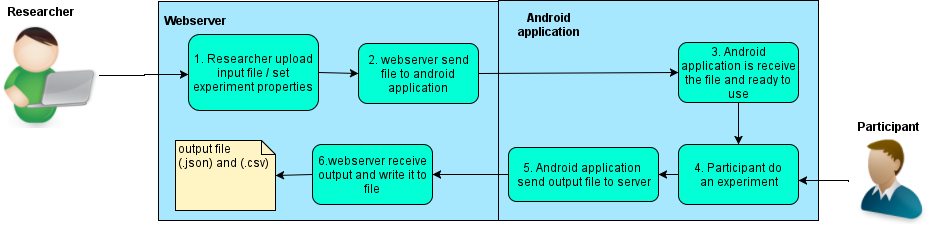
\includegraphics[width=\textwidth]{framework_process}
\centering
\captionsetup{justification=centering}
\caption{Flow of the experiment framework}
\label{fig:mainline}
\end{figure}

\subsection{Requirement}

The table \ref{tab:requirementList} below shows the list of all requirements of the application and its description.
% The main part are there are two
% main actors, a researcher and a participant. Researcher will able to set a input file and set parameters for the experiment. Participants then able to do the experiment by using the experiment application provided by the researcher. the application track the variables of the experiment. Finally, the researcher then able to download the experiment output\\

\begin{table}[!b]
  \centering
  \small
  \footnotesize
	\begin{tabu}{ |X[0.5,l]|X[5,l]|X[9,l]|  }
     \hline
     \multicolumn{3}{|c|}{Requirement List} \\
     \hline
     No& Name & Text \\
     \hline
     1   & Upload Input    & Researcher upload a JSON input file to the application\\ \hline
     2 & Download Output & Researcher download a JSON output file of the experiment\\ \hline
     3 & Insert multiple categories & Researcher insert multiple categories \\ \hline
     4 &  Insert questions & On each category researcher insert multiple questions\\ \hline
     5 & Set number of presented question & Researcher set how many question will be presented on each quiz phase   \\ \hline
     6 & Set presented question behavior &  Researcher set whether the number of presented question will be random each phase \\ \hline
     7 & Insert post question  &  Researcher insert the question that will be asked after the experiment, e.g demographic question \\ \hline
		 8 & Set experiment properties & Researcher able to set extra experiment's properties apart from input file.\\ \hline
		   9 & Insert notification  &  Researcher insert notifiaction and information on
       what is its content, when it will appear\\ \hline
       % and ow many millisecond  it takes to wait before shown to the user
      9 & See the questions  &  The participant can see the questions\\ \hline
      10 & Show answer link and answer page &  The participant can see and able to click the answer links  \\ \hline
      11 & Fill the answer  &  The participant can write an answer\\ \hline
      12 & Show notification  &  The application can show the notification \\ \hline
      13 & Track variables  &  The application can track defined variables\\
    \hline
    \end{tabu}
 \caption{List of requirements}
 \label{tab:requirementList}
\end{table}


\subsection{Input and Output}


The researcher needs to upload the input file that consist of all the experiment properties. After the experiment finish, the result can be downloaded as a JSON file.
JSON (Java Script object notation) is used as an input and output format because it is very easy for a human to read and write, also for the machine to parse and generate.
Most of the current programming language and analysis software support JSON format \citep{jsonDesc}.
The JSON format consist of key and value pairs, on many language it is similar to dictionary, table or struct. This input file will then be uploaded and compiled to the android application.
Here is a simple example of the JSON format. 
%\hfill \break
%\newline
% \noindent\fbox{%
%     \parbox{\textwidth}{%
%        \{\\
%     \hspace{10mm}    name :"John",\\
%    \hspace{10mm}     age:21,\\
%     \hspace{10mm}    hooby:swimming\\
%        \}
%        }
%     }%
% \hfill \break
\begin{lstlisting}[language=json,firstnumber=1]
 {
    name:"John",
    age:21,
    hobby:"swimming"
 }
\end{lstlisting}
The table \ref{tab:inputFile} shows all the field for the input and its description. The output of the application will be a JSON file that consist of the experiment result
which consist of the answer of the all the questions and tracked variables.



\subsection{Application Entities}
The input file that the researcher uploaded will be generated to an object.
The architecture of the object can be seen in figure \ref{fig:Experiment_objects}.
 Each box represents an object that consist of properties and methods.


 The biggest object is a \textit{study} object, this object is acted as a container for other objects.
The \textit{study} object holds another objects and control the flow of the experiment. The arrow in figure \ref{fig:Experiment_objects} represent which \textit{experiment}, \textit{category},
\textit{questions} and \textit{notification} will be used on the experiment. The \textit{study} object also acts as a tracker which will tracks variables during the experiment.

The \textit{experiment} object consists of properties on how the experiment will works, e.g experiment name, number of question will be asked, and how the question will be presented.
And each \textit{category} objects consist of \textit{questions} objects.

The researcher is able to choose which \textit{experiment} will be used and which \textit{notification} will be appeared.
While the participant can choose which \textit{category} they want to answered.
This selected \textit{experiment} and \textit{category} objects will be linked by
\textit{study} object and compiled as \textit{active category},\textit{active question} and \textit{active experiment}.

\begin{figure}[!b]
\begin{center}
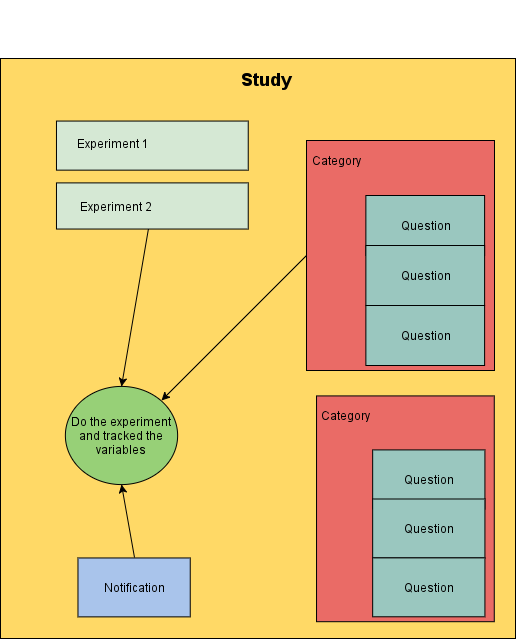
\includegraphics[scale=0.5]{quiz_Diagram}
\end{center}
\centering
\captionsetup{justification=centering}
\caption{Structure of the object inside the application}
\label{fig:Experiment_objects}
\end{figure}


\subsection{Application flow and properties}

The application have a general properties describe on the table \ref{tab:variableList} which will be used to identify the status of the experiment.
These properties is also used to decide which notifications to show and what variables to track.

Figure \ref{fig:quiz_flowchart} shows the flow chart of the quiz experiment, and how the application properties is updated.
Figure \ref{fig:quiz_flow} shows the front end the application when the participant do the quiz experiment.

To make it easier for the reader the experiment's flow is divided into four stages;
\begin{figure*}[!b]
\begin{multicols}{2}
    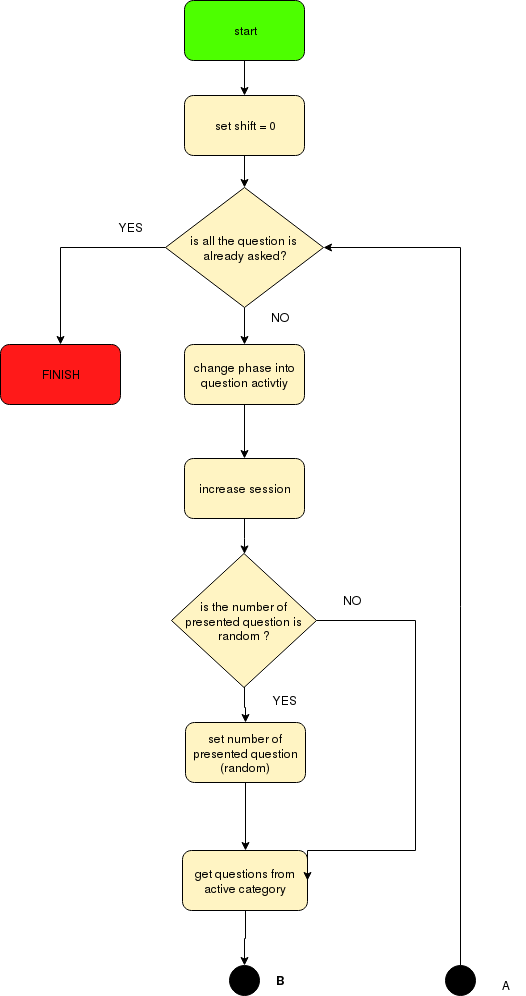
\includegraphics[scale=0.4]{Quiz_activity}\par
    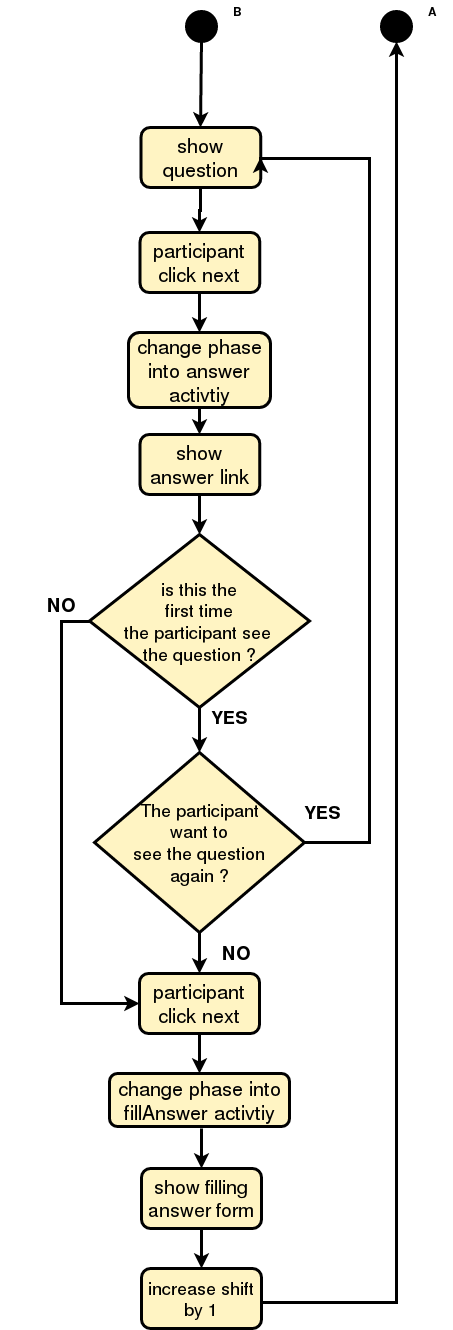
\includegraphics[scale=0.35]{Quiz_Activity_2}\par
    \end{multicols}
\centering
\captionsetup{justification=centering}
\caption{Quiz flowchart}
\label{fig:quiz_flowchart}
\end{figure*}


\begin{figure}[!t]
\begin{center}
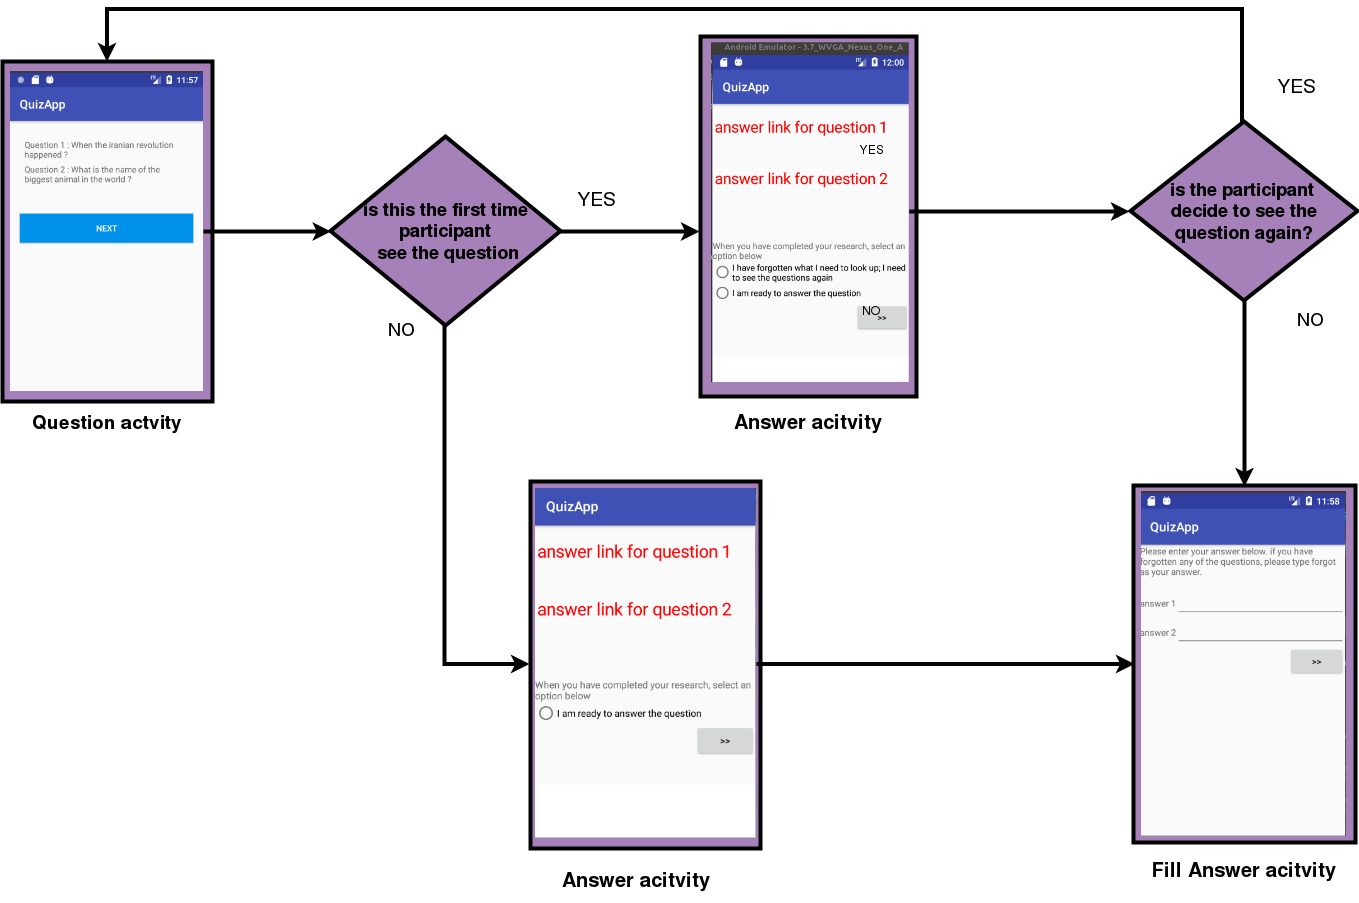
\includegraphics[scale=0.3]{Quiz_flow}
\end{center}
\centering
\captionsetup{justification=centering}
\caption{Front end of quiz activity flow}
\label{fig:quiz_flow}
\end{figure}

% \begin{itemize}
% \item \textit{Shift} : This variable is used to count how many question-answer had been done.
% \item \textit{Phase} : this variable has a value on what activity is currently active on the application
% \item \textit{Active Category} : The active category that will be choose by the participant during the experiment. This category will contain list of questions.
% \item \textit{Active Experiment} : This variable will contains the properties of the current experiment, this properties is set by the researcher from the application
% \item \textit{Number of presented question} : this variable value shows how many question are asked at one \textit{shift} of question-answer.
% \item \textit{Active Question }: the current question and it's answer link that is presented to the participant. This active question is picked from the question list inside the active category. the number of active question is based on \textit{number of presented question} variable.
% \end{itemize}

\begin{table}[!b]
  \centering
  \small
  \footnotesize
	\begin{tabu}{ |X[0.5,l]|X[3,l]|X[3,l]|X[7,l]|  }
		\hline
     No& Properties name & Type & Function \\
     \hline
     1   & \textit{Shift} & Integer & Used to count how many question-answer had been presented.\\ \hline
     2 & \textit{Phase} & String & What the name of activity that is currently active on the application.\\ \hline
     4 & \textit{Active Category} & Category & Contain category used in the experiment, and it contains list of questions.  \\ \hline
     5 &  \textit{Active Experiment} & Experiment & Contains the properties of the current experiment. \\ \hline
     %The properties is set by the researcher from the application.\\ \hline
     6 & \textit{Number of presented question} & Integer &  How many questions are presented at a time (\textit{shift}). \\ \hline
7 & \textit{Active Question } & List of Question & List of the question that is presented to the participant. \\
                        %This variable is picked from the question list inside the active category.\\
\hline
    \end{tabu}
    % \centering
    % \captionsetup{justification=centering}
 \caption{List of general properties of the experiment}
 \label{tab:variableList}
\end{table}



\begin{itemize}
\item \textbf{Initialization} : firstly a \textit{phase} variable is initialize. The application then check if the experiment is active by ensuring that there is still questions need to be asked. The quiz is finished if all the question has been asked.
\item \textbf{Question activity} :  The number of presented question is changed (randomly or constant).
Then questions are picked from the \textit{active category} and put to \textit{active question}. Then the \textit{active questions} are presented to the participant.
\item \textbf{Answer activity} : Thirdly, the links for the answer page are presented to the participant. The participant then click the links and find the answer inside the answer page.
The participant is able see the question again or decide to answer. The participant are only allowed to see the question again one time.
\item \textbf{fill answer activity} Lastly, the participant need to write the answer of the question on the text box.
After that, the \textit{phase} variable is increased and the application will repeat the quiz again until it finished.
\end{itemize}


\subsection{Notification Design}

During the quiz experiment the notification will be shown to the participant.
Notification will be shown as a pop-up box as seen in figure \ref{fig:clicked_notification_flow}.
When the notification is poped up to the screen, the phone will vibrate and produce a sound.

 If the participant click the notification then the application will be minimized and the android phone will be directed to another application.
 After that, the user can click the application icon to get back to the experiment application.

Based on this design, the \textit{notification} should have the properties listed on table \ref{NotifactionProperties}.
% \begin{itemize}
% \item \textit{shift} : This property is to decide on which shitft the notification will be shown, it will be compared to the \textit{shift} properties of the study object.
% \item \textit{phase} : This properties is to decide on which activity (question, answer and fill answer) the notification will be shown.
% \item \textit{app} : What application the notification will open, it also need to have a value of the user or url of the application.
% \item \textit{timeToshow} : How millisecond the framework should wait before the notification will be shown
% \item \textit{notification text} : What is the message text inside the notification box
% \end{itemize}

\begin{table}[!b]
\centering
\small
\footnotesize
\begin{tabu}{|X[2,l]|X[5,l]|}
\hline
Variable          & Function                                                                                                                                  \\ \hline
shift             & This property is to decide on which shitft the notification will be shown, it will be compared to shift variable in experiment properties \\ \hline
phase             & This properties is to decide on which activity (question, answer and fillanswer) the notification will be shown.                          \\ \hline
app               & An application the notification will open; instagram, twitter, facebook or website.                           \\ \hline
timeToshow        & Time (in millisecond) notificationwill the notifiaction need to wait before presented.                                                           \\ \hline
notification text & The message text inside the pop-up box                                                                                     \\ \hline
\end{tabu}
% \centering
% \captionsetup{justification=centering}
\caption{The properties of notification object}
\label{NotifactionProperties}

\end{table}


\begin{figure}[!b]
\begin{center}
\fbox{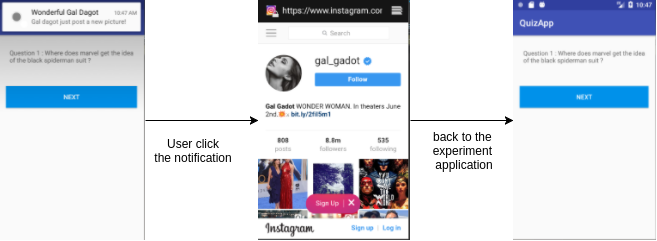
\includegraphics[scale=0.65]{notication}}
\end{center}
\centering
\captionsetup{justification=centering}
\caption{Flow of the notification}
\label{fig:clicked_notification_flow}
\end{figure}



\subsection{Tracked Variable}
During the experiment the application track variables. Table \ref{tab:trackedVarible} consist of all the variables that the application track.
some of the variable has \textbf{lb} in front of their name, this mean that variable is tracked during the lookback process.
A process when the participant look the question again for the second time.

\begin{table}[!b]
  \centering
  \small
  \footnotesize
\begin{tabu}{ |X[0.3,l]|X[2.3,l]|X[0.9,l]|X[5,l]|  }
 \hline
 \multicolumn{4}{|c|}{Tracked variables list} \\
 \hline
 No & Variable's name & Type & Description \\
 \hline
 1 & TTLQ & Long  & total time (in millisecond) when the participant see the question until they click next button\\ \hline
 2 & lb\_TTLQ & Long & similar with TTLQ, but after lookback\\ \hline
 3 & LookBack & Boolean & \textbf{True} if the participant decide to look at the question again, \textbf{false} otherwise. \\ \hline
 4 & TTLB & Long & total time (in millisecond) when the participant see the answer links until they click the next button (to look the question again or answer the question) \\ \hline
 5 & lb\_TTLB & Long & Similar with TTLB, but after lookback\\ \hline
 6 & visited\_links & List of String & The list of links clicked/visited by the participant after clicking the answer links\\ \hline
 7 & time\_visited\_links & List of Long  & List of the total time (in millisecond) the participant spent on each asnwer page\\ \hline
 8 & lb\_visited\_links & List of String & Similar to visited\_links, but after lookback\\ \hline
 9 & lb\_time\_visited\_links & List of Long & Similar with time\_visited\_links, but after lookback\\ \hline
 10 & TTLA & Long & Total time (in millisecond) the participant spent writing the answer\\
 11 & TTLFA & Long & Total time (in milisecond) the participant write the answer on the text box\\ \hline
 12 &  num\_notif & Integer & how many notification is shown during the a question \\ \hline
 13 & TTLN & Long & Total time (in millisecond) it tooks the participant after clicking the notification to back to experiment application\\ \hline
 \end{tabu}

%
%  \hline
%  \end{longtable}
\caption{List of tracked variable}
 \label{tab:trackedVarible}
\end{table}
\par
